\ifdefined\DIPLOMA
    \subsubsection{Техническое задание}

    Спроектировать малый привод манипулятора, устанавливаемого на малом спутнике
    съёмки Земли (рис. \ref{sattelite_general_view}).
\else
    \subsection{Назначение и общий вид манипулятора}

    Целью данной курсовой работы ставится проектирование одного из двух
    приводов манипулятора, устанавливаемых на малых спутниках съемки Земли
    (рис. \ref{sattelite_general_view}).
\fi

Манипулятор представляет собой двухзвенный электроприводной механизм,
предназначенный для скоростного наведения оптических камер.
Задачей манипулятора является организация перенацеливания камеры в заданное положение.

\begin{figure}[h!]
    \centering
    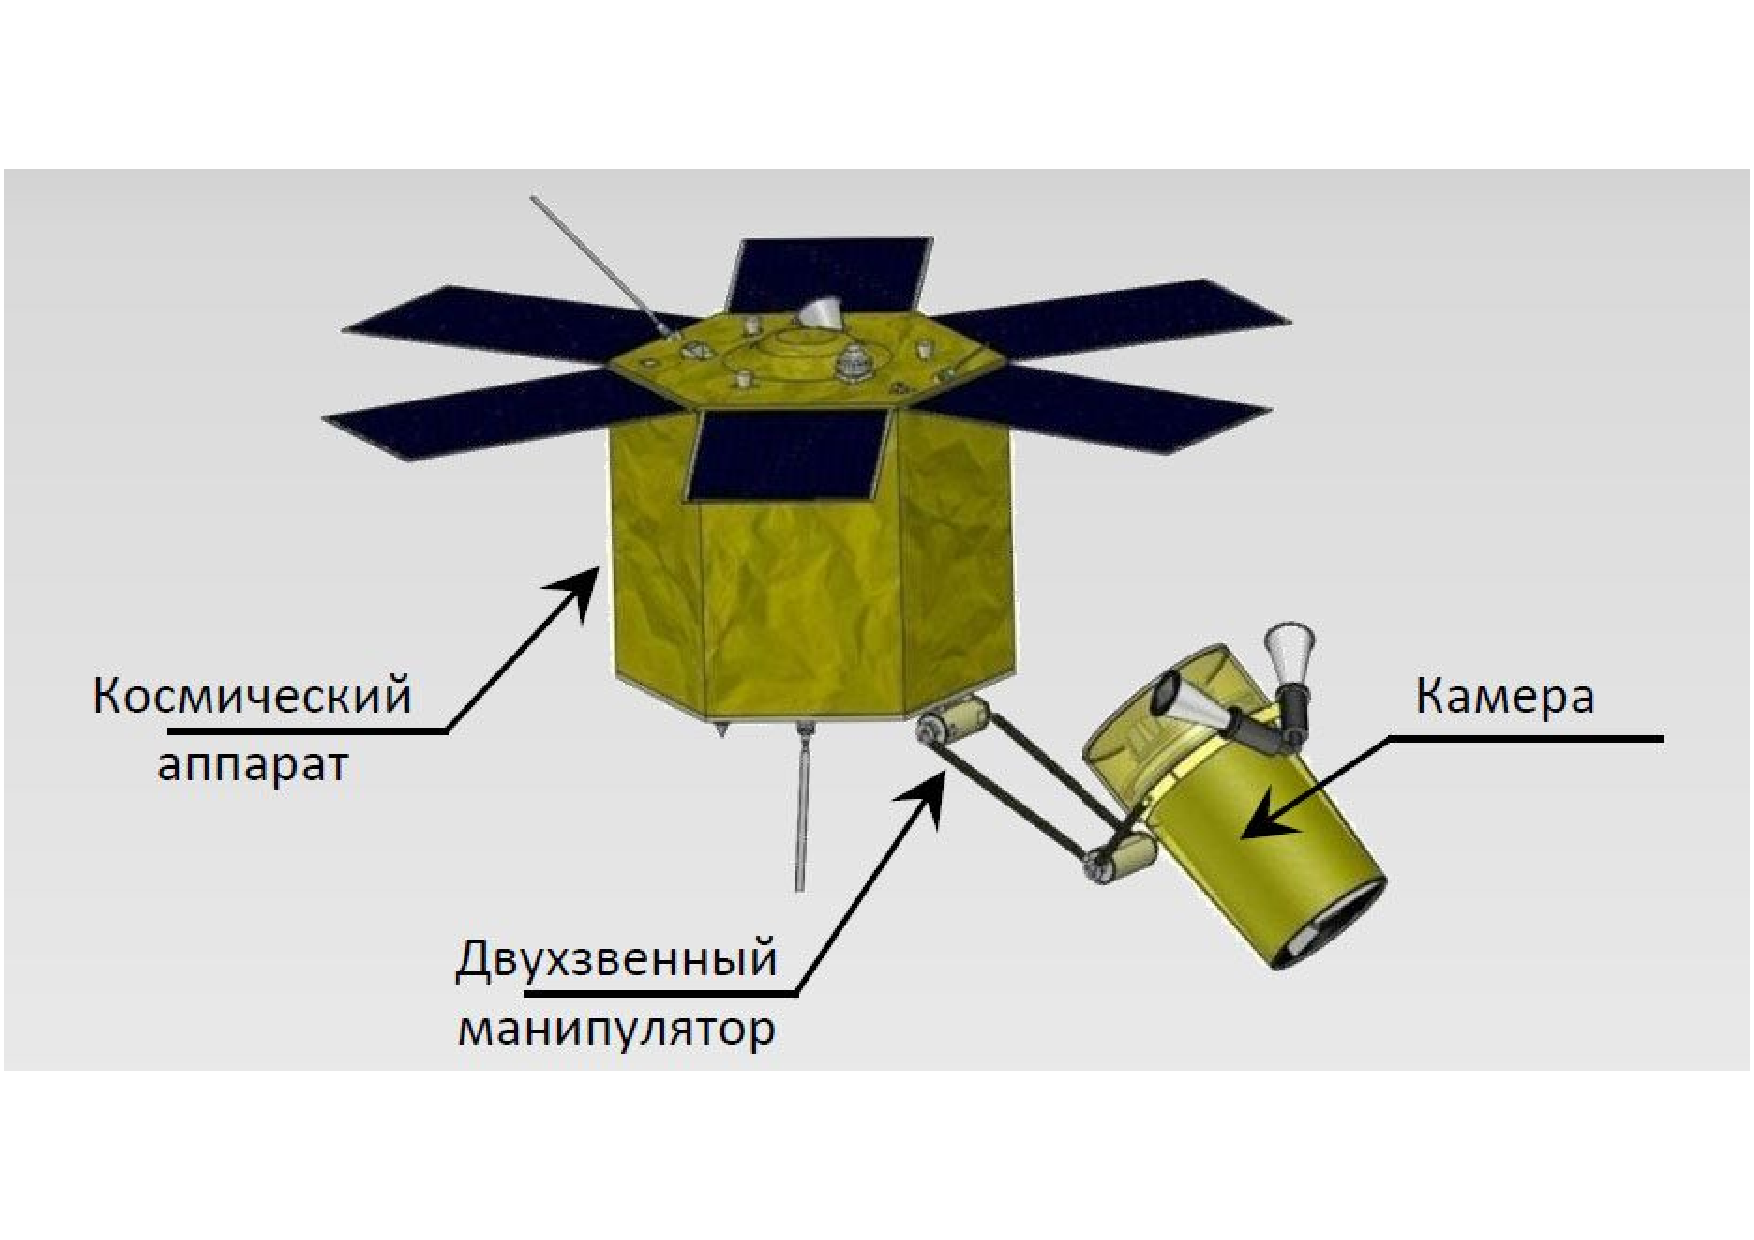
\includegraphics[width=\textwidth, keepaspectratio, clip=true, trim=3cm 3cm 3cm 3cm]
                    {./src/pictures/sattelite_3d_images/general_view}
    \caption{Манипулятор наведения камеры малого спутника Земли}
    \label{sattelite_general_view}
\end{figure}

Программные движения манипулятора осуществляются с помощью двух электроприводных блоков,
обеспечивающих поворот камеры в одной плоскости (в плоскости перпендикулярной
вектору движения космического аппарата по орбите).

Максимальный диапазон углового перенацеливания камеры: $\beta_{max} = -45..+45^{\circ}$.
Привод должен обеспечивать режимы переброски удовлетворяющие следующим 3--м движениям:

\begin{enumerate}
    \item Перенацеливание камеры на $q = 20^{\circ}$ за $t_{\textit{п}} = 2  $ c
    \item Перенацеливание камеры на $q = 45^{\circ}$ за $t_{\textit{п}} = 3  $ c
    \item Перенацеливание камеры на $q = 90^{\circ}$ за $t_{\textit{п}} = 4.3$ c
\end{enumerate}

В данный момент манипуляторы подобного рода на спутниках широко востребованы
в областях картографирования, планировки территорий, образовательных,
разведывательных и военных целях, метеорологии и т.п.

К подобным манипуляторам предъявляют высокие требования по точности,
надежности, массе, габаритам.

В качестве объекта проектирования был выбран малый привод, непосредственно вращающий камеру.

\endinput
